\documentclass[class=minimal, border = 0pt, crop]{standalone}
\usepackage{pgf}
\usepackage{tikz}
\usepackage[utf8]{inputenc}
\usetikzlibrary{arrows,automata,shapes,calc, backgrounds}
\usetikzlibrary{positioning}
\pagestyle{empty}
\tikzset{
    state/.style={
           rectangle,
           rounded corners,
           draw=black, very thick,
           minimum height=2em,
           inner sep=5pt,
           text centered,
           },
    pil/.style={
           ->,
           thick,
           shorten <=4pt,
           shorten >=4pt,
           },
    ball/.style={
           circle,
           draw,
           align=center,
           anchor=north,
           inner sep=0,
           fill=black,
           }
}

\begin{document}
\centering
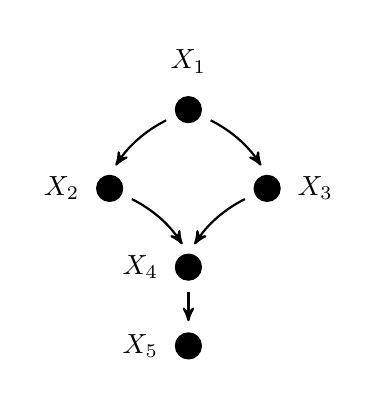
\begin{tikzpicture}[->,>=stealth']
\tikzstyle{every node}=[draw,shape=circle, fill=black]
\node (a1) at (0,0) [label=above:$X_1$] {};
\node (a2) at (-1,-1) [label=left:$X_2$] {};
\node (a3) at (1,-1) [label=right:$X_3$] {};
\node (a4) at (0,-2) [label=left:$X_4$] {};
\node (a5) at (0,-3) [label=left:$X_5$] {};
\path (a1) edge[pil, bend right = 15] (a2.north);
\path (a1) edge[pil, bend left = 15] (a3.north);
\path (a2) edge[pil, bend left = 15] (a4.north);
\path (a3) edge[pil, bend right = 15] (a4.north);
\path (a4) edge[pil] (a5.north);
\path (a5) edge[pil,color = white, bend right = 15] (a3.south);
\end{tikzpicture}
\end{document}